\section{Примери имплементација}

\subsection{\textit{Augmented reality offloading}}

У овом примеру тема је апликација за проширену стварност која у реалном времену камером анализира околину и детектује познате објекте. Апликација, на снимку уживо, препознатим објектима задебљава спољну ивицу како би се лакше уочили на слици \ref{fig:ar_example}.

\begin{figure}[H]
    \centering
    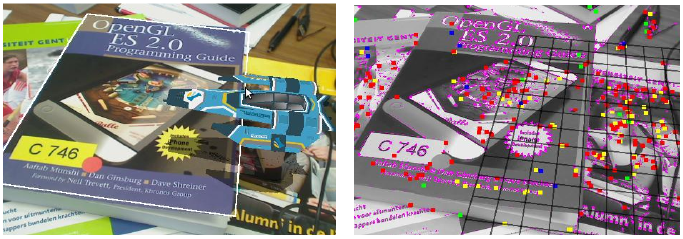
\includegraphics[width=1\textwidth]{images/ar_example.png}
    \caption{Са десне стране приказан је међукорак у раду апликације, док се на левој страни може приметити оивичена књига коју је апликација препознала}
    \label{fig:ar_example}
\end{figure}

Будући да је ова апликација намењена за коришћење у покрету, мобилни телефони се намећу као идеални уређаји за ову намену, али они сами по себи не поседују довољно хардверских ресурса за захтевна процесирања у реалном времену која су неопходна за несметан рад. Такође, делегирање читавог процесирања рачунарима на \textit{cloud}-у није адекватно због великог времена одзива, које не иде у корист обради у реалном времену. У даљем тексту биће описан процес разлагања апликације на независне процесе који се затим распоређују на \textit{cloudlet }aрхитектуру уређаја која се налази  близу уређаја на коме је покренута апликација.

\subsubsection{Разлагање апликације на процесе}

\begin{figure}[H]
    \centering
    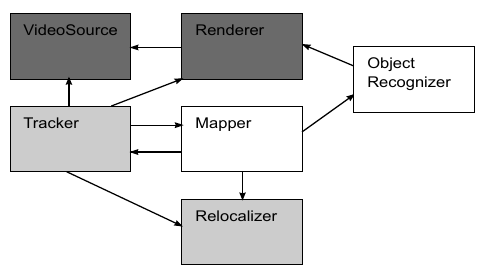
\includegraphics[width=1\textwidth]{images/ar_processes.png}
    \caption{Процеси од којих је сачињена апликација}
    \label{fig:ar_processes}
\end{figure}

На слици \ref{fig:ar_processes} може се приметити неколико процеса који заједно чине апликацију. \textit{Video source} представља камеру телефона која генерише видео садржај и прослеђује га \textit{Renderer}-у који преко њега поставља помоћну мрежу која је поравната са положајем камере који се прати уз помоћ \textit{Tracker}-а. Тако обрађене фрејмове \textit{Mapper} добија и покушава да пронађе и постави значајне тачке које су од помоћи \textit{Object recognizer}-у који на самом крају проналази и истиче објекте на слици. Улога \textit{Relocalizer}-a је да у случају да ниједна значајна тачка није пронађена на слици промени позицију камере како би се праћење наставило.


Сваки од наведених процеса има различите захтеве у погледу хардверских ресурса. \textit{Video source} и \textit{Renderer} се из јасних разлога морају налазити на мобилном уређају који пoкреће апликацију, док се остали процеси могу делегирати екстерним уређајима. \textit{Tracker} и \textit{Relocalizer} захтевају више хардверских ресурса као што је случај и са \textit{Mapper}-ом и \textit{Object recognizerom} с тиме да \textit{Tracker} и \textit{Relocalizer} морају имати много бржи одзив од преостала два. 


Како би било могуће покретати ове процесе на разним врстама уређаја, процеси су имплементирани у \textit{Java} програмском језику уз помоћ \textit{OSGi} сервисно оријентисаног система за управљање модулима. Имплементација процеса критичних по перформансе рађена је у \textit{C/C++}-у, а затим, због компатибилности са остатком система, обмотана \textit{Java} адаптером.

\subsubsection{\textit{Cloudlet} архитектура}

Претходно дефинисани процеси представљају основну компоненту овог система и они се покрећу унутар извршних окружења \textit{(EE)}. Више извршних окружења комуницира међусобно путем \textit{RPC} протокола. Процеси могу да дефинишу додатнa ограничења која се тичу перформанси у виду \textit{XML} шеме, где је то наjчешће брзина извршавања коју уређај на коме се процес извршава мора да испуни.  

\begin{figure}[H]
    \centering
    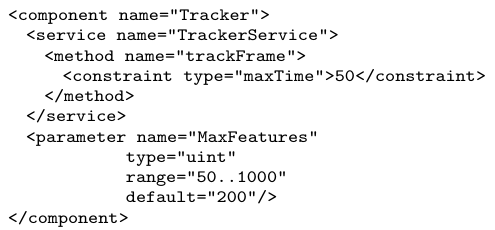
\includegraphics[width=1\textwidth]{images/cloudlet_constraints.png}
    \caption{Пример описа процеса који додатно намеће ограничења у виду брзине извршавања}
    \label{fig:cloudlet_constraints}
\end{figure}


Један или више извршних окружења покрећу се у оквиру једног оперативног система који је покренут на правом или виртуелизованом хардверу. Један овакав оперативни систем са покренутим извршним окружењима представља чвор и њиме управља \textit{node agent (NA)},  који управља извршним окружењима, креира нова и стопира их. \textit{node agent (NA)} такође надзире искориштење ресурса у оквиру комплетног чвора. 

Више чворова који се налазе физички близу једни других (имају малу међусобну латенцију), чине \textit{cloudlet}. \textit{Cloudlet}-ом управља  \textit{cloudlet agent} који комуницира са свим интерним \textit{node agent}-има. Више \textit{cloudlet}-а такође могу међусобно да комуницирају у циљу размене процеса. Унутар роја суседних чворова \textit{cloudlet agent} се покреће на чвору са највише ресурса.

За време извршавања, ако извршно окружење уочи да је ограничење неког од процеса прекршено, оно обавештава \textit{node agent}-а који даље обавештава \textit{cloudlet agent}-а који у том тренутку покушава да измени распоред процеса у оквиру његовог \textit{cloudlet}-а и тако оптимизује рад апликације. Оваква хијерархијска архитектура има неколико предности. Много је склабилније да једно тело унутар роја доноси одлуку о реорганизацији него да сваки чвор учествује у дистрибуираном гласању. Калкулисање расподеле посла увек се врши на чвору са највише ресурса и који има увид у све остале чворове, као и могућност комуникације са осталим \textit{cloudlet}-има.


Постоје две врсте \textit{cloudlet}-а, \textit{ad hoc} и еластични. \textit{ad hoc cloudlet} чине динамички пронађени чворови у локалној мрежи. Када се нови чвор придружи мрежи његов \textit{node agent} се активира и покреће извршна окружења, док \textit{cloudlet agent} врши ребалансирање посла при сваком уласку и изласку неког од чворова из мреже. Еластични \textit{cloudlet} се извршава на виртуализованој инфраструктури, где се чворови извршавају унутар виртуалних машина. У овом случају \textit{cloudlet agent} има могућност да креира и стопира чворове по потреби.

На слици \ref{fig:cloudlet_arch} може се видети пример горе описане архитектуре где \textit{ad hoc cloudlet} чинe десктоп рачунар, лаптоп и паметни телефон, док се еластични \textit{cloudlet} налази на јавној \textit{cloud} инфраструктури. 

\begin{figure}[H]
    \centering
    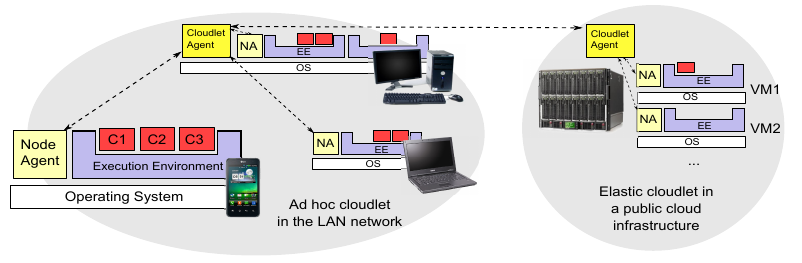
\includegraphics[width=1\textwidth]{images/cloudlet_arch.png}
    \caption{Пример \textit{cloudlet} архитектуре са еластичним и  \textit{ad hoc cloudlet}-има}
    \label{fig:cloudlet_arch}
\end{figure}

\pagebreak

\subsection{Обезбеђивање отпорности на отказе у здравственим установама}

У здравственим установама,  захтева се беспрекоран рад апликације. Ове апликације управљају критичним задацима као што су чување података о пацијентима, праћење њиховог тренутног стања и давање лекова. Сваки застој или квар може директно утицати на негу и безбедност пацијената.

\textit{Cloud} решења нуде скалабилност и лакоћу управљања за апликације у здравству, међутим постоје проблеми у вези са кашњењем, поузданошћу мреже, безбедношћу података као и несметаним наставком рада у случају отказа \textit{cloud} система или мрежних проблема. 

\textit{Fog computing} представља могуће решење ових проблема, коришћењем сензорских и серверских уређаја који се налазе у непосредној близини здравствене установе, тиме испуњавајући високе захтеве оваквог типа установе.

У конкретној имплементацији као адекватни механизам изабрана је реактивна отпорност на грешке детекцијом отказа ослушкивањем \textit{heartbeat} сигнала главног \textit{cloud} сервера и затим пребацивање на привремени \textit{fog} сервер као и реплицирану локалну базу података. Овакав приступ је изабран јер  крајњи корисници који се налазе на рубу мреже често могу имати проблема са конекцијом на главни сервер или немогућношћу повезивања услед његовог пада, док \textit{fog} сервер не пати од таквих проблема јер се налази у локалној мрежи. 

Читав систем састоји се из три модула: детекција отказа, репликација сервиса и делегирање посла резервном чвору. Као \textit{fog} уређај кориштен је \textit{Raspberry Pi 4}. 

Детекција отказа врши се ослушкивањем \textit{heartbeat} сигнала \textit{cloud} севера. Модул је имплементиран \textit{python} скриптом која на сваких 5 секунди шаље упит на адресу \textit{cloud} сервера. 

\begin{figure}[H]
    \centering
    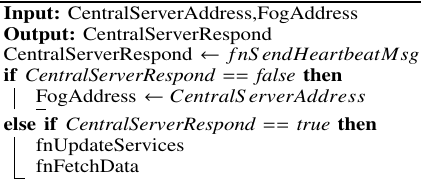
\includegraphics[width=1\textwidth]{images/db_update.png}
    \caption{Код за синхронизацију локалне базе података}
    \label{fig:db_update}
\end{figure}

Услед ограничених ресурса \textit{fog} уређаја, репликација сервиса своди се само на најважније и неопходне сервисе, што би био \textit{Apache Tomcat} сервис на коме се покреће \textit{backend Java Swing} апликација и \textit{MySQL} база података. Реплицирани сервис представља хладну реплику, што би значило да му се у току нормалног рада апликације корисници уопште не обраћају, све док je могућ приступ примарном сервису. База података синхронизује се са главном базом података на прилично стандардан начин \ref{fig:db_update}, где \textit{python} скрипта периодично шаље упит главној бази података и уколико је она доступна, подаци се ажурирају, а уколико није \textit{fog} бази се додељује адреса налик централној и на тај начин крајњи корисници не примећују било какву промену у случају пада базе података.



Делегирање посла са главног сервера на \textit{fog} сервер врши се по сличном принципу као и синхронизација бази података, где у случају недоступности главног сервера \textit{fog} сервер поставља као своју адресу адресу главног сервера и преузима посао,  с тиме да наставља да ослушкује \textit{heartbeat} сигнал главног сервера како би му вратио контролу када се његово стање стабилизује. Исти алгоритам користи се и за делегирање посла у случају преоптерећења главног сервера. \ref{fig:ip_switching}

\begin{figure}[H]
    \centering
    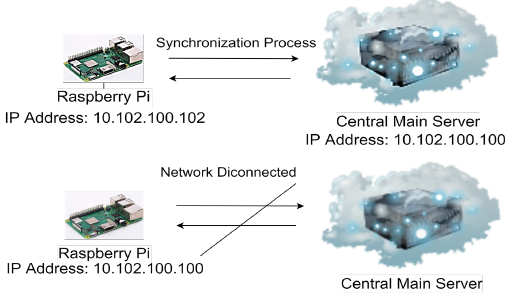
\includegraphics[width=1\textwidth]{images/ip_switching.png}
    \caption{Илустрација рада система када је главни сервер у и ван функције}
    \label{fig:ip_switching}
\end{figure}